

\setchapterpreamble[c][.7\textwidth]{\itshape\color{gray}\small
    Relationen setzen die Elemente einer Menge untereinander in Beziehung. Von besonderer Bedeutung sind Ordnungs- und Äquivalenzrelationen, deren grundlegende Sprache in diesem Vortrag entwickelt und an Beispielen verdeutlicht wird.
\vspace{24pt}}


\chapter{Relationen} \label{chap:relationen}


\section{Allgemeines}


Dieses Kapitel handelt von einer mathematischen Abstraktion des bereits im Logikkapitel in \cref{def:praedikat} eingeführten Relationenbegriffs.


\begin{defin}[Relation] \label{def:relation} \index{Relation}
    Sei $X$ eine Menge. Eine (zweistellige) \textbf{Relation auf $X$} ist ein mathematisches Objekt, das mit zwei beliebigen Elementen von $X$ zu einer Aussage kombiniert werden kann.

    Sind $R$ eine Relation auf $X$ und $x,y\in X$ zwei Elemente, so notieren wir die sich ergebende Aussage mit
        \[ xRy \]
    und sagen: „$x$ steht in der Relation $R$ zu $y$“.
\end{defin}


\begin{axiom}[* Gleichheit von Relationen] \label{relgleich}
    Seien $X$ eine Menge und $R,S$ zwei Relationen auf $X$. Genau dann stimmen $R$ und $S$ überein, wenn hinsichtlich $R$ und $S$ genau dieselben Elemente in Relation zueinander stehen. Als Formel:
        \[ R=S \qquad\Leftrightarrow\qquad (\forall x,y\in X:\quad xRy\ \leftrightarrow\ xSy) \]
    Vergleiche dieses Axiom mit \cref{mengengleich}, \cref{familiengleich} und \cref{abbgleich}.
\end{axiom}


\begin{nota}[Relationen definieren]
    Seien $X$ eine Menge und $E(a,b)$ ein zweistelliges Prädikat, für dessen beide Variablen jeweils alle Elemente von $X$ eingesetzt werden können. Der Ausdruck
    \begin{align*}
        xRy \quad &:\Leftrightarrow\quad E(x,y) && x,y\in X
    \end{align*}
    ist als eine Definition zu verstehen: es wird eine Relation $R$ auf $X$ definiert mit der Eigenschaft, dass für $x,y\in X$ die Aussage $xRy$ äquivalent zu $E(x,y)$ sei. Wegen \cref{relgleich} ist die Relation $R$ durch diese Eigenschaft eindeutig bestimmt\footnote{vgl. \cref{def:extension} und \cref{def:zuordnung}}. Der Buchstabe $R$ dient hierbei als \textbf{Relationssymbol}.
\end{nota}


\begin{bsp} \label{bsp:relation} \index{Teiler} \index{Vielfaches} \quad
    \begin{enumerate}
        \item(Verwandtschaftsgrade) Sei $M$ die Menge aller Menschen. Auf $M$ gibt es beispielsweise die Relationen:
        \begin{align*}
            xKy \qquad&:\Leftrightarrow\qquad x\ \text{ist ein Kind von}\ y && \\
            xNy \qquad&:\Leftrightarrow\qquad x\ \text{ist ein Nachfahre von}\ y && \\
            xGy \qquad&:\Leftrightarrow\qquad x\ \text{ist Bruder oder Schwester von}\ y && x,y\in M
        \end{align*}
        \item(Teilbarkeit) Man schreibt
        \begin{align*}
            m \mid n \qquad& :\Leftrightarrow\qquad \exists k\in \Z:\ k\cdot m=n && m,n\in \Z \\
            (\text{lies: „$m$ teilt $n$”})
        \end{align*}
        Dadurch wird eine Relation auf $\Z$ definiert, die \textbf{Teilbarkeitsrelation}. Sind $m,n\in \Z$ mit $m\mid n$, so heißen $m$ ein \textbf{Teiler} von $n$ und $n$ ein \textbf{Vielfaches} von $m$.
        \item(Teilmengenrelation) Auf der Gesamtheit aller Mengen gibt es die Teilmengenrelation $\subseteq$, die in \cref{def:teilmenge} definiert wurde.
        \item(Ordnung der Zahlbereiche) Auf $\N,\Z,\Q,\R$ gibt es die Relationen $\le, \ge, <, >$.
    \end{enumerate}
\end{bsp}


\begin{nota}[Negation einer Relation]
    Seien $X$ eine Menge, $R$ eine Relation auf $X$ und $x,y\in X$. Die Aussage, dass $x$ \emph{nicht} in Relation zu $y$ steht, wird in vielen Fällen mit einem durchgestrichenen Relationszeichen $R\mkern-11mu/$ notiert.
\end{nota}


\begin{bsp} \quad
    \begin{enumerate}
        \item Die Negation der Gleichheitsrelation $=$ ist die Ungleichheitsrelation $\neq$.
        \item Die Negation der Elementrelation $\in$ ist die Relation $\notin$ („kein Element von“).
        \item Die Negation der Teilmengenrelation $\subseteq$ ist die Relation $\nsubseteq$ („keine Teilmenge von“).
        \item Für $m,n\in \Z$ wird die Aussage, dass $m$ kein Teiler von $n$ ist, notiert mit $m\nmid n$.
    \end{enumerate}
\end{bsp}


\begin{defin}[Umkehrrelation] \label{def:umkehrrel} \index{Umkehrrelation}
    Seien $X$ eine Menge und $R$ eine Relation auf $X$. Die Relation $R^\op$, die definiert ist durch
    \begin{align*}
        xR^\op y \qquad &:\Leftrightarrow\qquad yRx && x,y\in X
    \end{align*}
    heißt die \textbf{Umkehrrelation} von $R$ (englisch: ``opposite relation''). 
\end{defin}


\begin{nota} \label{spiegelrel}
    Abseits allgemeiner theoretischer Überlegungen ist die Schreibweise $R^\op$ unüblich. Stattdessen wird die Umkehrrelation häufig mit dem gespiegelten Relationszeichen notiert.
\end{nota}


\begin{bsp}
    Die Umkehrrelation\dots
    \begin{enumerate}
        \item \dots der Teilmengenrelation $\subseteq$ ist die Obermengenrelation $\supseteq$, d.h. für Mengen $M,N$ gilt:
            \[M\supseteq N \iff N\subseteq M \]
        \item \dots der „kleinergleich“-Relation $\le$ ist die „größergleich“-Relation $\ge$.
    \end{enumerate}
\end{bsp}


\begin{bem}[*]
    Für jede Relation $R$ gilt $(R^\op)^\op=R$, d.h. die Umkehrrelation der Umkehrrelation von $R$ ist wieder $R$ selbst.
\end{bem}
\begin{proof}
    Sei $X$ eine Menge mit einer Relation $R$. Für alle $x,y\in X$ gilt:
        \[ x(R^\op)^\op y \quad\Leftrightarrow\quad yR^\op x \quad\Leftrightarrow\quad xRy  \]
    Weil $x,y\in X$ beliebig gewählt waren, folgt aus \cref{relgleich}, dass $(R^\op)^\op = R$.
\end{proof}


\begin{defin}[Eingeschränkte Relation] \label{def:einschraenkungrelation} \index{Einschränkung einer Relation}
    Seien $X$ eine Menge, $R$ eine Relation auf $X$ und $U\subseteq X$ eine Teilmenge. Dann ist durch
    \begin{align*}
        x\ R\vert_U\ y \qquad& :\Leftrightarrow\qquad xRy &&x,y\in U
    \end{align*}
    eine Relation auf $U$ definiert, die \textbf{Einschränkung von $R$ auf $U$} oder auch die \textbf{von $X$ vererbte Relation}. Die eingeschränkte Relation $R\vert_U$ stimmt quasi mit $R$ überein, mit dem einzigen Unterschied, dass sie nur noch auf die Elemente von $U$ angewandt wird.
\end{defin}


\begin{bsp}
    Die gewöhnlichen $\le$-Relationen auf $\N$, $\Z$ und $\Q$ sind allesamt Einschränkungen der $\le$-Relation auf $\R$. Denn eine natürliche/ganze/rationale Zahl $x$ ist genau dann kleinergleich eine andere solche Zahl $y$, wenn $x\le y$ im Sinne reeller Zahlen gilt.
\end{bsp}


\begin{bem}[* Pullback von Relationen] \label{pullbackrel}
    Seien $X,Y$ zwei Mengen, $X\xrightarrow{f} Y$ eine Abbildung und $R$ eine Relation auf $Y$. Dann ist durch
    \begin{align*}
        a\ f^*R\ b \qquad& :\Leftrightarrow\qquad f(a)\ R\ f(b) &&a,b\in X
    \end{align*}
    eine Relation „$f^*R$“ auf $X$ gegeben, der \emph{Pullback von $R$ entlang $f$} oder die \emph{entlang $f$ zurückgezogene Relation}.

    Im Spezialfall, dass $X\subseteq Y$ eine Teilmenge und $f=(X\xhookrightarrow{\iota_X} Y)$ die natürliche Inklusion sind, ist $\iota_X^*R=R\vert_X$ genau die Einschränkung von $R$ auf $X$. Das Konzept „Einschränkung einer Relation“ ist also ein Spezialfall des Konzepts „Pullback einer Relation“.
\end{bem}


\begin{bsp}[* feinere/gröbere Relation] \label{def:groebererelation} \index{feinere Relation} \index{groebere Relation@gröbere Relation}
    Seien $X$ eine Menge und $R,S$ zwei Relationen auf $X$. Die Relation $R$ heißt \textbf{feiner} als die Relation $S$ (und $S$ heißt \textbf{gröber} als $R$), wenn gilt
    \begin{align*}
        xRy \ &\implies\ xSy && \text{für alle}\ x,y\in X
    \end{align*}
    also wenn je zwei Elemente, die in Relation $R$ zueinander stehen, auch in Relation $S$ zueinander stehen.

    Bezeichnet $\Rel(X)$ die Menge aller Relationen auf $X$, so haben wir auf $\Rel(X)$ also eine „ist feiner als“-Relation.
\end{bsp}


\begin{vorschau}[* mengentheoretische Relationsdefinition]
    Die Relationsdefinition \cref{def:relation} ist, ähnlich wie die Mengendefinition \cref{def:menge} und die Abbildungsdefinition \cref{def:abbildung}, rein axiomatisch. Wenn man denn möchte, lässt sie sich aber durch eine präzise mengentheoretische Definition ersetzen:
    \begin{quote}
        Eine Relation auf einer Menge $X$ ist eine Teilmenge $R\subseteq X\times X$. Für Elemente $x,y\in X$ definiert man:
        \begin{align*}
            xRy\qquad:\Leftrightarrow\qquad (x,y) \in R
        \end{align*}
    \end{quote}
    Vermöge dieser Definition wird \cref{relgleich} zu einer beweisbaren Aussage und die „ist feiner als“-Relation aus \cref{def:groebererelation} wird schlicht zur Teilmengenrelation auf $\calP(X\times X)$. Für die Praxis ist sie aber wenig relevant. Stattdessen erfolgt der Umgang mit Relationen über diejenigen Prädikate, die sie definieren.
    
    Beachte, dass nicht jede Relation durch einen einfachen sprachlichen Ausdruck gegeben sein muss. Prinzipiell können Relationen beliebig kompliziert oder gar nicht mehr sprachlich beschreibbar sein. Beim Übergang vom syntaktischen Relationsbegriff aus \cref{def:praedikat} zum abstrakten Relationsbegriff aus \cref{def:relation} treten die gleichen Phänomene auf, die auch in \cref{zuordvsabb} beschrieben wurden.
\end{vorschau}


\begin{bsp}[Universelle Relationen] \label{def:universellerelationen} \index{Allrelation} \index{Leere Relation}
    Sei $X$ eine beliebige Menge.
    \begin{itemize}
        \item Die \textbf{Allrelation} auf $X$ ist diejenige Relation auf $X$, bei der jedes Element mit jedem Element in Relation steht. Sie entspricht der trivialen Teilmenge $X\times X\subseteq X\times X$.
        \item Die \textbf{leere Relation} ist diejenige Relation auf $X$, bei der kein Element mit irgendeinem anderen in Relation steht. Sie entspricht der leeren Teilmenge $\emptyset\subseteq X\times X$.
        \item Die \textbf{Gleichheitsrelation} auf $X$ ist die Relation $=$, bei der zwei Elemente genau dann in Relation stehen, wenn sie identisch sind.
    \end{itemize}
\end{bsp}


\begin{bem}[* Dualität zwischen Syntax und Semantik] \label{syntaxvssemantik} \index{Dualität zwischen Syntax und Semantik}
    Im Verlauf der letzten Kapitel wurde der Reihe nach sprachlich-syntaktischen Gebilden aus der Logik (Aussagen, Eigenschaften, Terme, Relationen im Sinne von \cref{def:praedikat}) semantisch-abstrakte Pendants (Wahrheitswerte, Mengen, Abbildungen, Relationen im Sinne von \cref{def:relation}) an die Seite gestellt. Dies ist kein Zufall und kommt von der intimen Verschränkung von Prädikatenlogik und Mengenlehre. Eine logische Sprache zur Beschreibung einer mathematischen Theorie sollte bereits in ihrer Grammatik gewisse Strukturen der Theorie reflektieren. Umgekehrt werden mathematische Theorien so entwickelt, dass sie der Beschreibung durch eine gegebene Sprache möglichst zugänglich sind. Dies ist die Dualität zwischen Syntax und Semantik. In der Tatsache, dass sich einerseits beinahe alle Mathematik in Prädikatenlogik formulieren lässt, und andererseits die Mengenlehre eine vollständige Interpretation der prädikatenlogischen Sprache zulässt, liegt der Grund für die breite Nutzbarkeit mengentheoretischen Denkens, das seit Beginn des 20. Jahrhunderts den populärsten Rahmen zur Formalisierung von Algebra und Analysis bereitstellt.\footnote{vgl. \cref{higherorder}} Nichtsdestotrotz wirst du bereits in den ersten Semestern an die Grenzen dieses Denkens stoßen, wenn es um den Gebrauch bestimmter Artikel (\emph{die} Menge der reellen Zahlen, \emph{der} Faktorraum $V/U$, etc.) für Objekte, die genau genommen gar nicht eindeutig bestimmt im Sinne von \cref{kennzeichnung} sind, geht.

    Einige Entsprechungen sprachlicher Gebilde und abstrakter mathematischer Objekte:
    \begin{center}
    \begin{tabular}{ccc}
        Syntax &\phantom{a}& Semantik \\
        \midrule
        Aussage && Wahrheitswert \\
        Eigenschaft && Teilmenge \\
        $\land$ und $\lor$ && $\cap$ und $\cup$ \\
        Term && Abbildung \\
        Termsubstitution && Verketten von Abbildungen \\
        Relationen nach \cref{def:praedikat} && Relationen nach \cref{def:relation}
    \end{tabular}
    \end{center}
    Diese Liste soll aber nur als suggestive Merkhilfe gelesen werden. \emph{Die eine} Syntax-Semantik-Dualität gibt es nicht, da sowohl aufseiten der Syntax viele verschiedene Kalküle (Einsortige und mehrsortige Prädikatenlogik, Lambda-Kalkül, infinitäre Logiken, usf.), als auch aufseiten der Semantik viele verschiedene Interpretationsweisen (mengentheoretische Modelle, kategorielle Semantik, Kripke-Joyal-Semantik, usf.) in Gebrauch sind, die alle mit ihrer eigenen Syntax-Semantik-Dualität aufwarten.
\end{bem}


\begin{defin}[Einige Eigenschaften von Relationen] \index{reflexive Relation} \index{transitive Relation} \index{symmetrische Relation} \index{antisymmetrische Relation}
    Seien $X$ eine Menge und $R$ eine Relation auf $X$. Dann heißt die Relation $R$
    \begin{itemize}
        \item \textbf{reflexiv}, falls für alle $x\in X$ gilt, dass $xRx$. Mit anderen Worten: jedes Element steht in Relation zu sich selbst.
        \item \textbf{transitiv}, falls für alle $x,y,z\in X$ mit $xRy$ und $yRz$ gilt, dass auch $xRz$.
        \item \textbf{symmetrisch}, falls für alle $x,y\in X$ mit $xRy$ auch $yRx$ gilt.
        \item \textbf{antisymmetrisch}, falls für alle $x,y\in X$ mit $xRy$ und $yRx$ gilt, dass $x=y$.
    \end{itemize}
    In Formeln liest sich das leichter:
    \begin{align*}
        \text{reflexiv:} \qquad &&& xRx && \text{für alle}\ x\in X \\
        \text{transitiv:} \qquad && (xRy\ \text{und}\ yRz) \implies\ & xRz && \text{für alle}\ x,y,z\in X\\
        \text{symmetrisch:} \qquad && xRy \implies\ & yRx && \text{für alle}\ x,y\in X \\
        \text{antisymmetrisch:} \qquad && (xRy\ \text{und}\ yRx) \implies\ & x=y && \text{für alle}\ x,y\in X
    \end{align*}
\end{defin}


\begin{bem}
    Symmetrische Relationen können ebensogut über die Formel
    \begin{align*}
        xRy\quad & \iff \quad yRx && \text{für alle}\ x,y\in X
    \end{align*}
    definiert werden (also mit $\iff$ anstelle von $\implies$). Denn wenn \emph{für alle} $x,y\in X$ aus $xRy$ schon $yRx$ folgt, so folgt auch aus $yRx$ schon $xRy$, weil die Rollen von $x$ und $y$ einfach vertauscht werden können.

    Eine Relation ist genau dann symmetrisch, wenn sie mit ihrer Umkehrrelation übereinstimmt.
\end{bem}


\begin{bsp}[Verwandtschaftsgrade]
    Sei $M$ die Menge aller Menschen.
    \begin{enumerate}
        \item Die Relation „\dots ist ein Kind von \dots“ ist nicht reflexiv, da niemand sein eigenes Kind sein kann. Ebenso ist sie nicht symmetrisch, da meine Eltern nicht meine Kinder sind. Schließlich ist sie auch nicht transitiv, da, abgesehen von inzestuösen Verhältnissen, die Enkel eines Menschen $x$ keine Kinder von $x$ sind.
        \item Die Relation „\dots ist ein Nachfahre von \dots“ ist dagegen transitiv, weil die Nachfahren der Nachfahren eines Menschen $x$ ebenfalls Nachfahren von $x$ sind. Symmetrisch ist sie allerdings nicht.
        \item Die Relation „\dots ist Bruder oder Schwester von \dots“ ist symmetrisch. Sofern wir jeden Menschen auch als Bruder bzw. Schwester von sich selbst ansehen, ist sie auch reflexiv und transitiv.
    \end{enumerate}
\end{bsp}


\begin{bsp}[symmetrisch vs. antisymmetrisch]
    Die Eigenschaften „symmetrisch“ und „antisymmetrisch“ sind, anders als es die Wörter vielleicht vermuten lassen, keine Gegensätze.
    \begin{enumerate}
        \item Sei $X$ eine beliebige Menge. Sowohl die leere Relation als auch die Gleichheitsrelation auf $X$ sind zugleich symmetrisch und antisymmetrisch.
        \item Die Teilbarkeitsrelation auf $\Z$ ist weder symmetrisch (da etwa $2\mid 6$ aber $6\nmid 2$) noch antisymmetrisch (da etwa $4\mid -4$ und $-4\mid 4$, aber $4\neq -4$).
    \end{enumerate}
\end{bsp}


\begin{bem}[Die eigentliche Bedeutung der Transitivität] \label{kettenfalten}
    Seien $X$ eine Menge mit einer Relation $R$ und $a,b,c,d\in X$ eine Handvoll Elemente von $X$. Anstelle von „Es gilt $aRb$, $bRc$ und $cRd$“ schreibt man kurz\footnote{vgl. \cref{todotsto}}
        \[ aRbRcRd \]
    Beispielsweise schreibt man
        \[ \N \subseteq \Z\subseteq\Q\subseteq\R\subseteq \C \]
    oder
        \[ 2 < 4 < 8 < 12 < 15 \]
    Mit dieser Notation lässt sich die Definition der Transitivität durch folgende Formel ausdrücken:
    \begin{align*}
        xRyRz \ &\implies\ xRz && x,y,z\in X
    \end{align*}
    Transitivität heißt also, dass sich jede aus drei Gliedern bestehende Relationenkette „zusammenziehen“ lässt. Es lässt sich zeigen, dass dies bei transitiven Relationen auch für beliebig lange Ketten gilt. Für $n\in \N_{\ge 1}$ und $x_1,\dots , x_n\in X$ gilt:
    \begin{align*}
        x_1R \ldots Rx_n \ &\implies\ x_1Rx_n && (\text{sofern $R$ transitiv ist})
    \end{align*}
    Im Spezialfall, dass $R$ die Gleichheitsrelation ist, hast du das auch schon in der Schule andauernd ausgenutzt: Sind $x_1,\dots , x_n$ irgendwelche Zahlen/Vektoren/Funktionen/etc., so gilt
        \[ x_1=\ldots = x_n \ \implies\ x_1=x_n\]
    Beachte, dass diese Schlussfolgerung bei nicht-transitiven Relationen unzulässig ist. Beispielsweise gilt
        \[ 2\cdot 6 \neq 3\cdot 6\neq 3\cdot 4 \]
    aber die Folgerung, dass deswegen auch $2\cdot 6\neq 3\cdot 4$ gälte, wäre falsch. Ungleichheit von Zahlen ist keine transitive Relation.
\end{bem}


\begin{satz}[* Stabilität unter Umkehrung und Einschränkung] \label{releigstabil}
    Seien $X$ eine Menge, $R$ eine Relation auf $X$ und $E$ eine der vier Eigenschaften „reflexiv“, „transitiv“, „symmetrisch“, „antisymmetrisch“. Dann gilt:
    \begin{enumerate}
        \item Besitzt $R$ die Eigenschaft $E$, so besitzt auch die Umkehrrelation $R^\op$ die Eigenschaft $E$.
        \item Besitzt $R$ die Eigenschaft $E$, so besitzt für jede Teilmenge $U\subseteq X$ auch die Einschränkung $R\vert_U$ die Eigenschaft $E$.\footnote{Allgemeiner sind die drei Eigenschaften „reflexiv“, „transitiv“ und „symmetrisch“ jeweils „stabil unter Pullback“, d.h. jeder Pullback einer Relation mit einer dieser drei Eigenschaften besitzt ebenfalls diese Eigenschaft. Vgl. \cref{merkmal}.}
    \end{enumerate}
\end{satz}
\begin{proof} \quad
    \begin{enumerate}
        \item (Reflexivität): Sei $R$ reflexiv. Für jedes $x\in X$ gilt dann  $xRx$, also auch $xR^\op x$. Damit ist auch $R^\op$ reflexiv.

        (Transitivität): Seien $R$ transitiv und $x,y,z\in X$ mit $xR^\op yR^\op z$. Also gilt $zRyRx$ und aus der Transitivität von $R$ ergibt sich $zRx$, also $xR^\op z$. Da $x,y,z\in X$ beliebig gewählt waren, ist damit gezeigt, dass auch $R^\op$ transitiv ist.

        (Symmetrie): Ist $R$ symmetrisch, so ist $R^\op=R$, sodass auch $R^\op$ symmetrisch ist.

        (Antisymmetrie): Seien $R$ antisymmetrisch und $x,y\in X$ mit $x R^\op y$ und $y R^\op x$. In Termen von $R$ heißt das $y Rx$ und $x Ry$, sodass sich $y=x$ aus der Antisymmetrie von $R$ ergibt. Also ist $x=y$, sodass auch $R^\op$ antisymmetrisch ist.
        \item Bei den Definitionen von Reflexivität, Transitivität, Symmetrie und Antisymmetrie handelt es sich jeweils um Allaussagen über die Elemente von $X$. Wenn diese Aussagen für alle Elemente von $X$ gelten, so erst recht auch für alle Elemente der Teilmenge $U$. \qedhere
    \end{enumerate}
\end{proof}





\section{Ordnungsrelationen} \label{sec:ordnungsrelationen}


\begin{nota}
    Bisher habe ich allgemeine Relationen mit dem Buchstaben „$R$“ notiert. Ordnungsrelationen sind Verallgemeinerungen der bekannten „$\le$“-Relation auf den Zahlräumen $\N,\Z,\Q,\R$, weshalb eine allgemeine Ordnungsrelation meist mit dem Zeichen $\le$ notiert wird. Beachte allerdings, dass eine Ordnungsrelation im Allgemeinen nichts mit den herkömmlichen Ordnungen auf $\N,\Z,\Q,\R$ zu tun haben muss!
\end{nota}


\begin{defin}[Ordnungsrelation] \label{def:ordnungsrelation} \index{Ordnungsrelation} \index{Halbordnung} \index{Partielle Ordnung} \index{Geordnete Menge}
    Sei $X$ eine beliebige Menge. Eine Relation $\le$ auf $X$ heißt \textbf{Ordnungsrelation} (auch: \emph{partielle Ordnung} oder \emph{Halbordnung}\footnote{aber diese Bezeichnungen sind mir verhasst, weil sie den Irrtum nahelegen, Ordnungsrelationen seien irgendwie „unvollständig“ und könnten und sollten zu Totalordnungen (\cref{def:totalordnung}) „vervollständigt“ werden.}), wenn sie reflexiv, transitiv und antisymmetrisch ist. In Formeln:
    \begin{align*}
        & (\text{O1}) & \forall x\in X:&&\quad &x\le x && (\text{Reflexivität}) \\
        & (\text{O2}) & \forall x,y,z\in X:&&\quad (x\le y\quad \text{und}\quad y\le z)\ \implies\ & x\le z && (\text{Transitivität}) \\
        & (\text{O3}) & \forall x,y\in X:&&\quad  (x\le y\quad \text{und}\quad y\le x)\ \implies\ & x=y && (\text{Antisymmetrie})
    \end{align*}
    Eine \textbf{geordnete Menge} ist ein Paar $(X,\le)$, bestehend aus einer Menge $X$ und einer Ordnungsrelation $\le$ auf $X$. Sofern die Ordnungsrelation im Kontext klar oder gleichgültig ist, spricht man auch schlicht von „der geordneten Menge $X$“.
\end{defin}


\begin{bsp} \quad
    \begin{enumerate}
        \item Die herkömmliche „kleinergleich“-Relation $\le$ ist eine Ordnungsrelation auf $\R$, $\Q$, $\Z$ und $\N$. Sprechen Mathematiker von „der geordneten Menge $\R$“, so ist damit in der Regel die geordnete Menge $(\R,\le)$ gemeint.
        \item(Teilmengenrelation) Sei $M$ eine beliebige Menge. Dann ist die Teilmengenrelation $\subseteq$ eine Ordnungsrelation auf $\calP(M)$. Dies wurde in \cref{teilmengeneig} bewiesen. Somit ist $(\calP(M),\subseteq)$ eine geordnete Menge. Sofern nicht anders erwähnt, werde ich $\calP(M)$ fortan stets mit der Teilmengenordnung ausstatten. Ist von „der geordneten Menge $\calP(M)$“ die Rede, so ist damit die geordnete Menge $(\calP(M),\subseteq)$ gemeint.
        \item(* Fortsetzung und Einschränkung) Seien $X,Y$ zwei Mengen und\footnote{Zur Definition von $\bigsqcup$ siehe \cref{def:disjunktcup}.}
            \[ \Sigma := \smashoperator[r]{\bigsqcup_{A\in \calP(X)}} \Abb(A,Y) \]
        Für $(A,f),(B,g)\in\Sigma$ sei
        \begin{align*}
            (A,f) \le (B,g) \qquad:\Leftrightarrow\qquad A\subseteq B\quad \text{und}\quad g\vert_A=f
        \end{align*}
        Mit anderen Worten: $(A,f)\le (B,g)$ genau dann, wenn $g$ eine Fortsetzung von $f$ ist im Sinne von \cref{def:fortsetzung}. Dann ist durch $\le$ eine Ordnungsrelation auf $\Sigma$ gegeben.
    \end{enumerate}
\end{bsp}


\begin{nota} \label{striktkleiner}
    Sei $(X,\le)$ eine geordnete Menge. Für $x,y\in X$ schreibt man\footnote{vgl. die $\subsetneq$-Relation aus \cref{def:teilmenge}}
    \begin{align*}
        x \ge y \qquad &:\Leftrightarrow\qquad y \le x \\
        x < y \qquad &:\Leftrightarrow\qquad x\le y\quad \text{und}\quad y \not \le x \\
        x > y \qquad &:\Leftrightarrow\qquad y < x
    \end{align*}
    Es sind $\ge$ und $>$ per Definition genau die Umkehrrelationen von $\le$ und $<$ im Sinne von \cref{def:umkehrrel}.

    Für $a\in X$ verwende ich gerne folgende Notation:
    \begin{align*}
        X_{\le a} & := \{x\in X\mid x\le a\} & X_{\ge a} & := \{x\in X\mid x\ge a\}
    \end{align*}
    und analog sind $X_{<a}$ und $X_{>a}$ definiert. Zum Beispiel ist $\R_{>0}$ die Menge der positiven reellen Zahlen und $\N_{\ge 1}$ die Menge der bei Eins beginnenden natürlichen Zahlen.
\end{nota}


\begin{satz} \label{umkehrordnung}
    Sei $(X,\le)$ eine geordnete Menge. Dann gilt:
    \begin{enumerate}
        \item Die Umkehrrelation $\ge$ ist ebenfalls eine Ordnungsrelation auf $X$, die sogenannte \textbf{Umkehrordnung}.
        \item Für jede Teilmenge $U\subseteq X$ ist die Einschränkung von $\le$ auf $U$ ebenfalls eine Ordnungsrelation, die \textbf{auf $U$ induzierte Ordnung} oder \textbf{von $X$ geerbte Ordnung}.
    \end{enumerate}
\end{satz}
\begin{proof}
    Dies ergibt sich direkt aus \cref{releigstabil}.
\end{proof}


\begin{bem} \quad
    \begin{itemize}
        \item Ist $U$ eine Teilmenge einer geordneten Menge, so wird meist auch $U$ stillschweigend als geordnete Menge angesehen. Beispielsweise trägt die Menge der positiven reellen Zahlen $\R_{>0}$ die von $\R$ geerbte Ordnung, was in der Regel nicht nochmal explizit erwähnt wird.
        \item Die Relationen $<$ und $>$ sind keine Ordnungsrelationen, weil sie nicht reflexiv sind. An der Uni sehen wir die Relation $\le$ als „primär“ und die Relation $<$ als daraus abgeleitet an.\footnote{Die einzige mir bekannte Ausnahme stellt die Theorie der \href{https://en.wikipedia.org/wiki/Well-founded_relation}{fundierten Relationen} dar, wo $<$ wichtiger als $\le$ ist und Induktionsbeweisen zugrundeliegt.}
    \end{itemize}
\end{bem}


\begin{bsp}[* Präordnungen] \index{Praeordnung@Präordnung}
    Eine Relation heißt \textbf{Präordnung}, wenn sie reflexiv und transitiv ist (aber nicht unbedingt antisymmetrisch). Jede Ordnungsrelation ist eine Präordnung. Beispiele für Präordnungen, die keine Ordnungsrelationen sind:
    \begin{enumerate}
        \item(Teilbarkeit) Die Teilbarkeitsrelation auf $\Z$ ist eine Präordnung, d.h. reflexiv und transitiv, aber keine Ordnungsrelation, weil sie nicht antisymmetrisch ist.
        \begin{proof}
            (reflexiv): Für jede ganze Zahl $n\in \Z$ ist $1\cdot n=n$, sodass $n\mid n$.

            (transitiv): Seien $l,m,n\in \Z$ mit $l\mid m\mid n$. Demzufolge gibt es $r,s\in \Z$ mit $rl=m$ und $sm=n$. Es folgt
                \[ n = s\cdot m = s\cdot (r\cdot l) = (s\cdot r)\cdot l \]
                sodass auch $l\mid n$. Da $l,m,n\in\Z$ beliebig gewählt waren, ist die Teilbarkeitsrelation also transitiv.

            (nicht antisymmetrisch): Wegen $-2=(-1)\cdot 2$ und $2=(-1)\cdot (-2)$ gilt $2\mid -2$ und $-2\mid 2$. Weil aber $2\neq -2$, ist die Teilbarkeitsrelation nicht antisymmetrisch.
        \end{proof}
        \item(Logische Implikation) Sei $\calA$ die Menge aller mathematischen Aussagen. Dann ist die Relation
        \begin{align*}
            A\le B \qquad &:\Leftrightarrow\qquad  \text{Es lässt sich beweisen, dass $A\to B$} && A,B\in \calA
        \end{align*}
        eine Präordnung, d.h. reflexiv und transitiv. Sie ist jedoch nicht antisymmetrisch und somit keine Ordnungsrelation.\footnote{Mittels Übergang zur \emph{Lindenbaum-Algebra} kann sie allerdings künstlich antisymmetrisch gemacht werden, vgl. \cref{bsp:lindenbaum}.}
        \begin{proof}
            (reflexiv): Die Reflexivität wurde in \cref{implikationref} bewiesen.

            (transitiv): Die Transitivität ergibt sich aus \cref{implikationtrans}.

            (nicht antisymmetrisch): Beispielsweise gilt für $x\in\R$ und die Aussagen $A:\Leftrightarrow\ x=4$ und $B:\Leftrightarrow\ 2x=8$, dass $A\to B$ und $B\to A$. Dennoch sind $A$ und $B$ zwei (äquivalente, aber) verschiedene Aussagen.
        \end{proof}
    \end{enumerate}
\end{bsp}


\begin{defin}[Hasse-Diagramm] \label{def:hasse} \index{Hasse-Diagramm}
    Sei $(X,\le)$ eine geordnete Menge, die nur endlich viele Elemente enthält. Ein \textbf{Hasse-Diagramm}\footnote{\href{https://de.wikipedia.org/wiki/Helmut_Hasse}{Helmut Hasse (1898-1979)}} von $X$ besteht aus:
    \begin{itemize}
        \item Für jedes Element von $X$ ein Knotenpunkt.
        \item Für je zwei verschiedene Elemente $a,b\in X$ mit $a<b$, für die es kein $x\in X$ mit $a<x<b$ gibt, ein Kantenstrich zwischen den Punkten $a$ und $b$. Außerdem soll das „größere“ Element $b$ in einer einheitlich festgelegten Richtung vom Punkt $a$, etwa oberhalb von $a$ oder rechts von $a$, eingezeichnet sein.
    \end{itemize}
\end{defin}


\begin{bsp} \label{bsp:hasse}
    Hier sind ein paar Beispiele für Hasse-Diagramme:
    \begin{enumerate}
        \item Die geordnete Menge $\{1,2,3,4,5\}$ (mit der gewöhnlichen, von $\N$ induzierten Ordnung) kann visualisiert werden durch:
        \[\begin{tikzcd}
            1 \ar[r, dash] & 2 \ar[r, dash] & 3 \ar[r, dash] & 4 \ar[r, dash] & 5
        \end{tikzcd}\]
        \item Die geordnete Menge $(\{\{1\},\{2\},\{1,2,3\},\{1,2,4\}\},\subseteq)$ sieht folgendermaßen aus:
        \[\begin{tikzcd}
            \{1,2,3\} && \{1,2,4\} \\
            && \\
            \{1\} \ar[uu, dash] && \{2\} \ar[uu, dash] \ar[lluu, dash] \ar[from=ll, to=uu, dash, crossing over]
        \end{tikzcd}\]
        \item Die geordnete Menge $(\{\{1\},\{2\},\{1,2\},\{1,2,3\},\{1,2,4\}\},\subseteq)$ hat die folgende Form:
        \[\begin{tikzcd}
            \{1,2,3\} && \{1,2,4\} \\
            & \{1,2\} \ar[lu, dash] \ar[ru, dash] & \\
            \{1\} \ar[ru, dash] && \{2\} \ar[ul, dash]
        \end{tikzcd}\]
        \item Die geordnete Menge $(\calP(\{1,2,3\}),\subseteq)$\footnote{vgl. \cref{bsp:potenzmenge}} sieht folgendermaßen aus:
        \[ \begin{tikzcd}
            & \{ 1,2,3 \} & \\
            \{ 1,2 \} \ar[ru, dash] & \{ 1,3\} \ar[u, dash] \ar[from = rd, dash] & \{ 2,3 \} \ar[lu, dash] \\
            \{ 1 \} \ar[u, dash] \ar[ru, dash] & \{ 2 \} \ar[lu, crossing over, dash] \ar[ru, crossing over, dash] & \{ 3 \} \ar[u, dash]\\
            & \emptyset \ar[lu, dash] \ar[ru, dash] \ar[u, dash] &
        \end{tikzcd} \]
        \item In manchen Fällen können auch geordnete Mengen mit unendlich vielen Elementen mit einer Art Hasse-Diagramm visualisiert werden. Beispielsweise lässt sich $(\Z,\le)$ darstellen als:
        \[\begin{tikzcd}
            \dots \ar[r, dash] & -2 \ar[r, dash] & -1 \ar[r, dash] & 0 \ar[r, dash] & 1 \ar[r, dash] & 2 \ar[r, dash] & \dots
        \end{tikzcd}\]
    \end{enumerate}
    Systematisch werden Hasse-Diagramme in der Drittsemester-Vorlesung „Algebra 1“ gezeichnet, wenn es um die Darstellung von \emph{Untergruppenverbänden} geht.
\end{bsp}


\begin{defin}[Vergleichbarkeit] \label{def:totalordnung} \index{Totalordnung} \index{vergleichbar (Ordnungstheorie)}
    Ist $(X,\le)$ eine geordnete Menge, so heißen zwei Elemente $x,y\in X$ miteinander \textbf{vergleichbar}, wenn $x\le y$ oder $y\le x$.

    Die Ordnungsrelation $\le$ heißt eine \textbf{Totalordnung}, wenn alle Elemente miteinander vergleichbar sind. Als Formel:
    \begin{align*}
        \le\ \text{ist eine Totalordnung}\qquad:\Leftrightarrow\qquad \forall x,y \in X:\quad x\le y\quad \text{oder}\quad y\le x 
    \end{align*}
    Ist $\le$ eine Totalordnung auf $X$, so heißt das Paar $(X,\le)$ eine \textbf{totalgeordnete Menge}.
\end{defin}


\begin{bsp}
    Es gilt:
    \begin{enumerate}
        \item $(\R,\le)$ ist eine totalgeordnete Menge, d.h. von je zwei reellen Zahlen ist stets die eine kleinergleich die andere. Ebenso sind auch $(\N,\le)$, $(\Z,\le)$ und $(\Q,\le)$ jeweils totalgeordnete Mengen.
        \item In der geordneten Menge $(\calP(\N),\subseteq)$ sind die Elemente $\{1\}$ und $\{1,2\}$ miteinander vergleichbar, da $\{1\}\subseteq \{1,2\}$. Die Elemente $\{1\}$ und $\{2\}$ sind dagegen nicht miteinander vergleichbar, da weder $\{1\}\subseteq\{2\}$ noch $\{2\}\subseteq \{1\}$ gilt.
        \item Allgemein gilt für eine beliebige Menge $M$ mit mindestens zwei verschiedenen Elementen, dass die geordnete Menge $(\calP(M),\le)$ nicht totalgeordnet ist. Allerdings besitzt sie die Struktur einer sogenannten \emph{Boolschen Algebra}.\footnote{vgl. \cref{bivalenz}}
    \end{enumerate}
\end{bsp}


\begin{bem} \quad
    \begin{enumerate}[a)]
        \item Die Umkehrordnung einer Totalordnung ist ebenfalls eine Totalordnung. Beispielsweise sind auch $(\N,\ge)$, $(\Z,\ge)$, $(\Q,\ge)$, $(\R,\ge)$ jeweils totalgeordnete Mengen.
        \item Jede Teilmenge einer totalgeordneten Menge ist mit der geerbten Ordnung ebenfalls totalgeordnet. Beispielsweise sind auch $\{n\in \N\mid n\ \text{ist ungerade}\}$ und das Intervall $[0,1]\subseteq\R$ jeweils totalgeordnete Mengen.
    \end{enumerate}
\end{bem}


\begin{bem}[Intuition für Totalordnungen]
    Das Hasse-Diagramm einer totalgeordneten Menge hat stets die Gestalt einer einzigen Linie. Aus diesem Grund werden Totalordnungen manchmal auch \emph{lineare Ordnungen} genannt. Allgemein hat sich für mich die Intuition bewährt, mir die Elemente einer totalgeordneten Menge $X$ „auf einem Streifen aufgereiht“ vorzustellen. Sind $x,y\in X$, so gilt, da $x$ und $y$ miteinander vergleichbar sind, dass $x\le y$ oder $y\le x$, also dass $x$ auf dem Streifen wahlweise links oder rechts von $y$ zu verorten ist.

    Für nicht-total geordnete Mengen versagt diese Intuition allerdings.
\end{bem}


\begin{defin}[Intervalle in $\R$] \label{def:intervall} \index{Intervall}
    Seien $a,b\in \R$ mit $a\le b$. Dann heißen
    \begin{itemize}
        \item $(a,b) := \{ x\in \R \mid a<x<b \}$ das \textbf{offene Intervall} mit den Randpunkten $a$ und $b$,
        \item $[a,b] := \{ x\in \R \mid a\le x\le b \}$ das \textbf{abgeschlossene Intervall} mit den Randpunkten $a$ und $b$.
        \item Die Mengen $[a,b) := \{ x\in \R \mid a\le x<b \}$ und $(a,b] := \{ x\in \R \mid a<x\le b \}$ heißen \textbf{halboffene Intervalle} mit Randpunkten $a$ und $b$. 
    \end{itemize}
    Das abgeschlossene Intervall $[a,b]$ unterscheidet sich vom offenen Intervall $(a,b)$ lediglich dadurch, dass in $[a,b]$ auch noch die beiden „Randpunkte“ $a$ und $b$ enthalten sind, während sie bei $(a,b)$ fehlen.

    Diese Definitionen ergeben auch Sinn, wenn man $\R$ durch eine beliebige geordnete Menge, wie z.B. die erweiterte Zahlengerade $\bar \R$ aus \cref{def:erweitertezahlengerade}, ersetzt.
\end{defin}


\begin{nota}[offene Intervalle vs. Paare]
    Das offene Intervall $(a,b)$ besteht also aus genau denjenigen Elementen, die zwischen $a$ und $b$ liegen. Es ist nicht zu verwechseln mit dem Paar $(a,b)\in \R^2$ aus \cref{def:tupel}. Da sowohl für das Paar $(a,b)\in \R^2$ als auch für das offene Intervall $(a,b)\subseteq \R$ dieselbe Notation verwendet wird, musst du beim Lesen mathematischer Texte aus dem Kontext ableiten, von welchem Objekt die Rede ist. Die bei manchen Autoren vorherrschende Schreibweise $]a,b[$ anstelle von $(a,b)$ werde ich nicht verwenden.
\end{nota}


\begin{defin} \label{def:kleinstes} \index{groesstes Element@größtes Element} \index{Maximum} \index{kleinstes Element} \index{Minimum} \index{maximales Element} \index{minimales Element}
Sei $X$ eine geordnete Menge. Ein Element $a\in X$ heißt
    \begin{itemize}
        \item \textbf{kleinstes Element} (oder auch: \textbf{Minimum}) von $X$, falls für jedes $x\in X$ gilt, dass $a\le x$. Mit anderen Worten: „Jedes Element ist größergleich $x$“.
        \item \textbf{größtes Element} (oder auch: \textbf{Maximum}) von $X$, falls für jedes $x\in X$ gilt, dass $x\le a$.
        \item \textbf{minimales Element} von $X$, falls es kein $x\in X$ gibt, für das $x<a$ gälte. Mit anderen Worten: „Es gibt kein strikt kleineres Element“.
        \item \textbf{maximales Element} von $X$, falls es kein $x\in X$ gibt, für das $a<x$ gälte.
    \end{itemize}
\end{defin}


\begin{satz}[Eindeutigkeit kleinster/größter Elemente] \label{kleinsteseind}
    Sei $X$ eine geordnete Menge. Sofern $X$ ein kleinstes bzw. größtes Element enthält, ist dieses eindeutig bestimmt.
\end{satz}
\begin{proof}
    Seien $a,b\in X$ zwei kleinste Elemente. Da $a$ ein kleinstes Element ist, gilt $a\le b$, und da $b$ ein kleinstes Element ist, gilt $b\le a$. Aus der Antisymmetrie von $\le$ folgt $a=b$.

    Die Aussage über größte Elemente wird analog bewiesen.
\end{proof}


\begin{nota}
    Dies rechtfertigt es, von \emph{dem} Minimum bzw. \emph{dem} Maximum von $X$ zu sprechen, im Sinne von \cref{kennzeichnung}. Notation:
    \begin{align*}
        \min(X) \qquad\text{und}\qquad \max(X)
    \end{align*}
    Beachte allerdings, dass ein kleinstes oder größtes Element nicht unbedingt existieren braucht.
\end{nota}


\begin{bsp} \label{bsp:kleinstes} \quad
    \begin{enumerate}
        \item $\N$ enthält ein kleinstes Element, nämlich die Null. Allerdings gibt es keine größte natürliche Zahl, denn für jedes $n\in \N$ ist $n+1>n$.
        \item Für jede beliebige Menge $M$ ist $\emptyset$ das kleinste und $M$ das größte Element von $(\calP(M),\subseteq)$.
        \item Die Menge $\R_{>0}$ der positiven reellen Zahlen enthält kein kleinstes Element. Dies wurde in \cref{bsp:widerspruchsbeweis} bewiesen.
        \item Die geordnete Menge $(\{\{1\},\{2\},\{1,2,3\},\{1,2,4\}\},\subseteq)$ enthält weder ein kleinstes noch ein größtes Element. Dennoch sind $\{1\}$ und $\{2\}$ jeweils minimale Elemente und $\{1,2,3\}$ und $\{1,2,4\}$ jeweils maximale Elemente.
        \item Auf jeder beliebigen Menge $X$ ist die Gleichheitsrelation $=$ eine Ordnungsrelation. Diesbezüglich ist \emph{jedes} Element sowohl minimal als auch maximal. Im Gegensatz zu kleinsten und größten Elementen brauchen minimale und maximale Elemente also nicht eindeutig sein.
    \end{enumerate}
\end{bsp}


\begin{satz} \label{kleinvsmin}
    Sei $X$ eine geordnete Menge. Dann gilt:
    \begin{enumerate}
        \item Jedes kleinste Element von $X$ ist auch ein minimales Element.
        \item Ist $X$ totalgeordnet, ist auch jedes minimales Element ein kleinstes Element.
    \end{enumerate}
    Analoge Aussagen gelten für größte und maximale Elemente.
\end{satz}
\begin{proof} \quad
    \begin{enumerate}
        \item Sei $a\in X$ ein kleinstes Element. Angenommen, es gäbe ein $x\in X$ mit $x<a$, also $x\le a$ und $a\not\le x$. Dann widerspräche $a\not\le x$ der Eigenschaft von $a$, ein kleinstes Element zu sein.
        \item Seien $X$ totalgeordnet und $a\in X$ ein minimales Element. Sei $x\in X$ beliebig. Es ist zu zeigen, dass $a\le x$. Weil $X$ totalgeordnet ist, gilt $a\le x$ oder $x\le a$, sodass eine Fallunterscheidung vorgenommen werden kann:
        \begin{enumerate}[1)]
            \item Im Fall $a\le x$ ist nichts mehr zu zeigen.
            \item Im Fall $x\le a$ folgt aus der Minimalität von $a$, dass auch $a\le x$ gelten muss.
        \end{enumerate}
        Also gilt in jedem Fall $a\le x$. Da $x$ beliebig gewählt wurde, ist somit $a$ ein kleinstes Element.
    \end{enumerate}
    Die Aussagen über größte und maximale Elemente werden analog bewiesen.
\end{proof}


\begin{bem}
    Im totalgeordneten Fall sind die Begriffe „Minimum“ und „minimales Element“ also gleichbedeutend. Vor allem der für die Analysis wichtige Fall $(\R,\le)$ ist davon abgedeckt. Dagegen zeigt \cref{bsp:kleinstes}, dass es im nicht-total geordneten Fall durchaus minimale Elemente geben kann, die kein Minimum sind. Die Terminologie von „Minimum“ und „minimalem Element“ ist unglücklich verwirrend und ich empfehle, das Wort „Minimum“ nur im totalgeordneten Fall zu verwenden und andernfalls von „kleinsten Elementen“ zu sprechen.
\end{bem}


\subsection*{Schranken}


\begin{defin}[Schranken] \label{def:schranken} \index{Schranke (Ordnungstheorie)} \index{beschränkt (Ordnungstheorie)}
    Seien $X$ eine geordnete Menge und $T\subseteq X$ eine Teilmenge. Ein Element $x\in X$ heißt
    \begin{itemize}
        \item eine \textbf{untere Schranke} für $T$, wenn für alle $t\in T$ gilt: $x\le t$.
        \item eine \textbf{obere Schranke} für $T$, wenn für alle $t\in T$ gilt: $t\le x$.
    \end{itemize}
    Die Teilmenge $T\subseteq X$ heißt
    \begin{itemize}
        \item \textbf{nach unten beschränkt} (in $X$), wenn es in $X$ mindestens eine untere Schranke für $T$ gibt.
        \item \textbf{nach oben beschränkt} (in $X$), wenn es in $X$ mindestens eine obere Schranke für $T$ gibt.
        \item \textbf{beschränkt} (in $X$), wenn sie sowohl nach oben als auch nach unten beschränkt ist.
    \end{itemize}
\end{defin}


\begin{bsp} \quad
    \begin{enumerate}
        \item Die Teilmenge $\N\subseteq \Z$ ist nach unten beschränkt, aber nicht nach oben beschränkt. Eine untere Schranke ist beispielsweise die Null. Ebenso ist jede negative Zahl eine untere Schranke.
        \item Sei $\bbP$ die Menge der Primzahlen. Nach dem Satz von Euklid \cref{euklid} besitzt $\bbP$ keine obere Schranke in $\N$.
        \item Das Einheitsintervall $[0,1]$ ist beschränkt in $\R$. Beispielsweise sind $1$ eine obere Schranke und $0$ eine untere Schranke.
    \end{enumerate}
\end{bsp}


\begin{bem} \quad
    \begin{itemize}
        \item Beachte, dass Beschränktheit ein „relativer“ Begriff ist: wir sprechen stets von der Beschränktheit von $T$ \emph{in $X$}. Beispielsweise ist das Intervall $(0,1]$ in $\R_{>0}$ nach unten unbeschränkt, da es keine positive Zahl gibt, die kleiner als jede Zahl zwischen $0$ und $1$ wäre. In $\R$ hingegen ist $(0,1]$ nach unten beschränkt, eine untere Schranke ist beispielsweise die $0$.
        \item Eine Teilmenge hat im Allgemeinen viele verschiedene Schranken. Beispielsweise ist jedes $x\in \R_{\le 0}$ eine untere Schranke für $(0,1]$. Allerdings ist die untere Schranke $0$ in gewisser Weise „optimal“, sie grenzt $(0,1]$ nach unten am engst möglichen ein.
    \end{itemize}
\end{bem}


\begin{defin}[Infimum und Supremum] \index{Infimum} \index{Supremum}
    Seien $X$ eine geordnete Menge und $T\subset X$ eine Teilmenge.
    \begin{itemize}
        \item Ein Element $a\in X$ heißt \textbf{Infimum} von $T$, wenn $a$ eine größte untere Schranke für $T$ ist. Das heißt, $a$ ist eine untere Schranke für $T$ und für jede weitere untere Schranke $x$ gilt $x\le a$.
        \item Ein Element $a\in X$ heißt \textbf{Supremum} von $T$, wenn $a$ eine kleinste obere Schranke für $T$ ist. Das heißt, $a$ ist eine obere Schranke für $T$ und für jede weitere obere Schranke $x$ gilt $a\le x$.
    \end{itemize}
\end{defin}


\begin{nota}
    Weil Infima und Suprema als kleinste bzw. größte Elemente gewisser Schrankenmengen definiert wurden, folgt aus \cref{kleinsteseind}, dass sie, sofern sie existieren, eindeutig bestimmt sind. Sofern die Teilmenge $T\subseteq X$ ein Infimum oder ein Supremum in $X$ besitzt, ist es, im Sinne von \cref{kennzeichnung}, also gerechtfertigt, von \emph{dem} Infimum bzw. \emph{dem} Supremum zu sprechen. Notation:
    \begin{align*}
        \inf(T) \qquad\text{und}\qquad \sup(T)
    \end{align*}
    Beachte allerdings, dass Infimum und Supremum nicht unbedingt existieren brauchen.

    Sofern sie existieren, gelten für jedes $x\in X$ folgende Äquivalenzen:
    \begin{align*}
        x\le \inf(T) \qquad&\Leftrightarrow\qquad \forall t\in T:\ x\le t \\
        \sup(T)\le x \qquad&\Leftrightarrow\qquad \forall t\in T:\ t\le x
    \end{align*}
    Dies sind zwei Beispiele für eine sogenannte \emph{universelle Eigenschaft}, die du dir einprägen solltest. In diesen beiden Ungleichungen ist die gesamte Definition von Infimum und Supremum kompakt kodiert.
\end{nota}


\begin{bsp} \quad
    \begin{enumerate}
        \item Weil $\N$ in $\Z$ nicht nach oben beschränkt ist, also gar keine einzige obere Schranke besitzt, besitzt $\N$ erst recht kein Supremum in $\Z$.
        \item Das offene Intervall $(0,1)\subseteq \R$ besitzt $0$ als Infimum und $1$ als Supremum. Allerdings sind $0,1\notin (0,1)$. Dieses Beispiel zeigt, dass das Infimum bzw. Supremum einer Teilmenge $T$ nicht unbedingt auch ein Element von ihr sein braucht. Wenn doch, handelt es sich um ein Minimum bzw. Maximum von $T$ im Sinne von \cref{def:kleinstes}.
        \item In der geordneten Menge $(\{\{1\},\{2\},\{1,2,3\},\{1,2,4\}\},\subseteq)$ (vgl.\cref{bsp:hasse}) besitzt die Teilmenge $T:=\{\{1\},\{2\}\}$ kein Supremum. Zwar besitzt sie genau zwei obere Schranken, nämlich $\{1,2,3\}$ und $\{1,2,4\}$, aber da keine der beiden kleiner als die andere ist, ist keine der beiden ein Supremum von $T$.
        \item In der geordneten Menge $(\{\{1\},\{2\},\{1,2\},\{1,2,3\},\{1,2,4\}\},\subseteq)$ (vgl. \cref{bsp:hasse}) besitzt die Teilmenge $T:=\{\{1\},\{2\}\}$ dagegen ein Supremum, nämlich $\{1,2\}$.
        \item Sei $M$ eine beliebige Menge. Dann besitzt jede Teilmenge $T\subseteq \calP(M)$ ein Infimum, nämlich $\bigcap T$ (wobei wir $\bigcap \emptyset:=M$ setzen) und ein Supremum, nämlich $\bigcup T$.\footnote{Geordnete Mengen, in denen jede endliche Teilmenge ein Infimum und ein Supremum besitzt, heißen \emph{Verbände}. Besitzt sogar \emph{jede} Teilmenge ein Infimum und ein Supremum, so spricht man von einem \emph{vollständigen Verband}. Das Beispiel zeigt, dass $(\calP(M),\subseteq)$ ein vollständiger Verband ist für jede beliebige Menge $M$.}
        \item Es ist $T:=\{x\in \Q \mid x^2 < 2\}$ eine beschränkte Teilmenge von $\Q$, die weder ein Supremum noch ein Infimum in $\Q$ besitzt. In $\R$ besitzt sie dagegen welche, nämlich $\sqrt{2}$ und $-\sqrt{2}$.
        \item Das \emph{Vollständigkeitsaxiom} besagt, dass jede nichtleere beschränkte Teilmenge von $\R$ ein Infimum und ein Supremum in $\R$ besitzt.
    \end{enumerate}
\end{bsp}


\begin{bem}[* Verallgemeinerbarkeit auf Präordnungen]
    Eine Analyse ergibt, dass sich alle Definitionen und nahezu alle Sätze aus diesem Abschnitt über Ordnungsrelationen verallgemeinern lassen auf sogenannte \emph{prägeordnete Mengen}, d.h. Mengen mit einer reflexiven und transitiven (aber nicht unbedingt antisymmetrischen) Relation. Die einzigen Aussagen, die im prägeordneten Fall nicht mehr gelten, sind die Eindeutigkeit kleinster und größter Elemente sowie die Eindeutigkeit von Infima und Suprema -- in die Eindeutigkeitsbeweise ging essenziell die Antisymmetrie ein.
\end{bem}


\begin{bem}[* Dualitätsprinzip für geordnete Mengen] \label{ordnungsdualitaet} \index{Dualitätsprinzip für geordnete Mengen}
    Nach \cref{umkehrordnung} ist für jede geordnete Menge $(X,\le)$ auch $(X,\ge)$ eine geordnete Menge. Zwischen $\le$ und der Umkehrordnung $\ge$ besteht eine weitreichende Dualität. Für eine Teilmenge $T\subseteq X$ sind beispielsweise die oberen Schranken von $T$ in der geordneten Menge $(X,\le)$ genau die unteren Schranken von $T$ in der geordneten Menge $(X,\ge)$. Man hat folgende Dualitätsbeziehungen:
    \begin{center}
    \begin{tabular}{ll}
        $(X,\le)$ & $(X,\ge)$ \\
        \midrule
        kleinstes Element & größtes Element \\
        minimales Element & maximales Element \\
        nach unten beschränkte Teilmenge & nach oben beschränkte Teilmenge \\
        untere Schranke & obere Schranke \\
        Infimum & Supremum
    \end{tabular}
    \end{center}
    Begriffe wie „vergleichbare Elemente“ sind sogar selbstdual, insofern zwei Elemente $x,y\in X$ genau dann in der geordneten Menge $(X,\le)$ miteinander vergleichbar sind, wenn sie vergleichbar sind in der Umkehrordnung $(X,\ge)$.

    Diese Dualität ist nicht nur eine nützliche Merkhilfe, sie spart uns auch eine Menge Beweisarbeit, insofern wir praktisch nur jede zweite Aussage über geordnete Mengen überhaupt beweisen müssen. Beispielsweise wurde in \cref{kleinvsmin} nur bewiesen, dass jedes kleinste Element ein minimales Element ist, mit der Anmerkung, der Beweis für die duale Aussage über größte und maximale Elemente „ginge analog“. Tatsächlich muss hier gar kein zweiter Beweis mehr geführt werden: Denn indem bewiesen wurde, dass in \emph{jeder} geordneten Menge $(X,\le)$ ein kleinstes Element auch ein minimales Element ist, gilt diese Aussage dann ja insbesondere auch für die geordnete Menge $(X,\ge)$. Aber die kleinsten und minimalen Elemente in $(X,\ge)$ sind genau die größten und maximalen Elemente in $(X,\le)$.
\end{bem}





\section{Äquivalenzrelationen} \label{sec:aequirel}


\begin{bem}[Philosophie der Äquivalenzrelationen] \label{aequirelphilo}
    Warum ist das Gleichheitszeichen $=$ eigentlich nicht überflüssig? Wir verwenden es, um auszudrücken, dass zwei Objekte identisch sind -- aber in diesem Fall ergibt es ja von vornherein überhaupt keinen Sinn, von \emph{zwei} Objekten zu sprechen. Beispielsweise ist die Gleichung
        \[ 12\cdot 18 = 6\cdot 36 \]
    gleichbedeutend zu $216=216$, also einer Information, die eigentlich nicht der Rede wert ist.
    
    Der springende Punkt ist hier das Vorliegen zweier verschiedener Abstraktionsebenen. Einerseits haben wir es beim Rechnen mit Zeichenketten wie „$12\cdot 18$“ oder „$6\cdot 36$“ zu tun. Auf einer abstrakteren Ebene interessieren wir uns für die Zahlen, die durch die Zeichenketten \emph{repräsentiert} werden. So sind etwa „$216$“\footnote{Beachte, dass auch der Ausdruck „$216$“ noch eine Abkürzung ist für „$2\cdot 10^2 + 1\cdot 10^1 + 6 \cdot 10^0$“.} und „$12\cdot 18$“ zwei \emph{verschiedene} Zeichenketten, die dennoch \emph{dieselbe} Zahl repräsentieren, und dies zu überprüfen erfordert Rechenaufwand. Es findet ein gedanklicher Abstraktionsprozess statt: zwei Objekte, die auf einer gewissen Ebene noch voneinander verschieden sind, fassen wir auf einer abstrakteren Ebene als identisch auf. Wir schwächen den Gleichheitsbegriff ab. Indem wir die Gleichung „$12\cdot 18=6\cdot 36$“ als nicht-selbstverständliche Aussage hinstellen, machen wir auf diesen Abstraktionsprozess aufmerksam.
    
    Formalisiert werden kann dieser Prozess durch Äquivalenzrelationen. Es handelt sich dabei um alternative Gleichheitsbegriffe, die schwächer als die herkömmliche, strikte Gleichheit sind, und dadurch eine „Gleichheit auf einer abstrakteren Ebene“ darstellen.

    Bisher wurden allgemeine Relationen mit dem Buchstaben $R$ und allgemeine Ordnungsrelationen mit dem Zeichen $\le$ notiert. Für allgemeine Äquivalenzrelationen nutze ich die Tilde $\sim$.
\end{bem}


\begin{defin}[Äquivalenzrelation] \label{def:aequirel} \index{Aequivalenzrelation@Äquivalenzrelation}
    Sei $X$ eine Menge. Eine Relation $\sim$ auf $X$ heißt \textbf{Äquivalenzrelation}, wenn sie reflexiv, symmetrisch und transitiv ist. In Formeln:
    \begin{align*}
        & (\text{ÄR1}) & \forall x\in X:&&\quad & x\sim x && (\text{Reflexivität}) \\
        & (\text{ÄR2}) & \forall x,y\in X:&&\quad x\sim y\ \implies\ & y\sim x && (\text{Symmetrie}) \\
        & (\text{ÄR3}) & \forall x,y,z\in X:&&\quad (x\sim y\ \text{und}\ y\sim z)\ \implies\ & x\sim z && (\text{Transitivität})
    \end{align*}
\end{defin}


\begin{bsp} \label{bsp:aequirel} \index{Kongruenz modulo $n$} \quad
    \begin{enumerate}
        \item(Gleichheit) Auf jeder beliebigen Menge $X$ ist die Gleichheitsrelation $=$ eine Äquivalenzrelation. Denn für beliebige $x,y,z\in X$ gilt:
        \begin{align*}
            & x = x \\
            x=y\quad \implies\quad & y=x \\
            (x=y\ \text{und}\ y=z) \quad\implies\quad & x=z
        \end{align*}
        \item(Äquivalenz von Aussagen) Sei $\calA$ die Menge aller mathematischen Aussagen. Dann ist die Relation
        \begin{align*}
            A\sim B \qquad&:\Leftrightarrow\qquad \text{Es lässt sich beweisen, dass $A\leftrightarrow B$} && A,B\in\calA
        \end{align*}
        eine Äquivalenzrelation auf $\calA$. Die Reflexivität wurde in \cref{iffref} bewiesen, die Symmetrie ergibt sich aus \cref{iffkomm} und die Transitivität folgt aus \cref{ifftrans}.
        \item(Kongruenz modulo $n$) Sei $n\in \N_0$. Die durch
        \begin{align*}
            a\equiv b\mod n \qquad& :\Leftrightarrow\qquad a-b\in n\Z && a,b\in \Z \\
            (\text{lies: „$a$ ist kongruent zu $b$ modulo $n$”})
        \end{align*}
        definierte Relation auf $\Z$ heißt \textbf{Kongruenz modulo $n$}. Per Definition sind zwei ganze Zahlen $a,b\in \Z$ genau dann kongruent modulo $n$, wenn ihre Differenz ein Vielfaches von $n$ ist. Beispielsweise gilt:
        \begin{alignat*}{6}
            16 &\equiv 1&\mod 5 \qquad&\qquad&\qquad  4 &\equiv 10 &\mod 3 \\
            -1&\equiv 1 &\mod 2 \qquad&\qquad&\qquad  5 &\equiv -4 &\mod 3 \\
            11 &\not\equiv 7 &\mod 5 \qquad&\qquad&\qquad 6 &\not\equiv 9 &\mod 4 \\
            85983 &\equiv 14238 &\mod 1 \qquad&\qquad&\qquad  1 &\equiv 0 &\mod 1 \\
            4 &\equiv 4 &\mod 0 \qquad&\qquad&\qquad  4 &\not \equiv 2 &\mod 0
        \end{alignat*}
        Die Kongruenz modulo $n$ ist eine Äquivalenzrelation.
        \item Auf jeder beliebigen Menge ist die Allrelation eine Äquivalenzrelation.
    \end{enumerate}
\end{bsp}


\begin{bem}[Gemeinsames Merkmal] \label{merkmal}
    Seien $X,Y$ zwei Mengen und $X\xrightarrow{f} Y$ eine Abbildung. Dann ist die Relation
    \begin{align*}
        a \sim_f b \qquad&:\Leftrightarrow\qquad f(a)=f(b) && a,b\in X
    \end{align*}
    eine Äquivalenzrelation auf $X$.\footnote{Es handelt sich genau um den Pullback der Gleichheitsrelation entlang $f$ im Sinne von \cref{pullbackrel}.} Stellen wir uns $f$ als eine Abbildung vor, die den Elementen von $X$ gewisse „Merkmale“ zuordnet, so formalisiert die Relation $\sim_f$ das Teilen solcher gemeinsamen Merkmale.
\end{bem}
\begin{proof}
    Alle Eigenschaften ergeben sich daraus, dass „$=$“ eine Äquivalenzrelation auf $Y$ ist:

    (Reflexivität): Für jedes $a\in X$ ist $f(a)=f(a)$, also $a\sim_f a$.

    (Symmetrie): Sind $a,b\in X$ mit $a\sim_f b$, also $f(a)=f(b)$, so ist auch $f(b)=f(a)$, also $b\sim_f a$.

    (Transitivität): Seien $a,b,c\in X$ mit $a\sim_f b\sim_f c$, d.h. $f(a)=f(b)=f(c)$. Es folgt $f(a)=f(c)$, sodass $a\sim_f c$.
\end{proof}


\begin{bsp} \quad
    \begin{enumerate}
        \item(Wohngemeinschaften) Sei $M$ die Menge aller Menschen, die genau eine Wohnung haben. Wir haben eine Abbildung $M\to \{\text{Wohnungen}\}$, die jeder Person aus $M$ ihre Wohnung zuordnet. Nach \cref{merkmal} ist also durch „lebt in derselben Wohnung wie“ eine Äquivalenzrelation auf $M$ gegeben. Im Detail heißt das:
        \begin{labeling}
            \item[(Reflexivität):] Jede Person wohnt mit sich selbst zusammen (so komisch das klingt).
            \item[(Symmetrie):] Wenn eine Person $A$ mit einer Person $B$ zusammenwohnt, so wohnt $B$ auch mit $A$ zusammen.
            \item[(Transitivität):] Wenn $A,B,C\in M$ drei Leute sind, bei denen $A$ mit $B$ und $B$ mit $C$ zusammenwohnt, so wohnt auch $A$ mit $C$ zusammen.
        \end{labeling}
        \item(Fußballvereine) Sei $F$ die Menge aller Fußballspieler in der Bundesliga. Wir haben eine Abbildung $F\to\{\text{Fußballvereine}\}$, die jedem Spieler seinen Verein zuordnet. Nach \cref{merkmal} ist also durch „spielt im selben Verein wie“ eine Äquivalenzrelation auf $F$ gegeben.
        \item Eine Konsequenz von \cref{aequiklassegleich} ist, dass sich \emph{jede} Äquivalenzrelation über die Konstruktion aus \cref{merkmal} realisieren lässt. Insofern jede Äquivalenzrelation ein Pullback einer Gleichheitsrelation ist, ist $=$ die „universelle Äquivalenzrelation“.
    \end{enumerate}
\end{bsp}


\begin{defin}[Äquivalenzklasse] \label{def:aequiklasse} \index{Aequivalenzklasse@Äquivalenzklasse} \index{Vertreter} \index{Repräsentant}
    Seien $X$ eine Menge, $\sim$ eine Äquivalenzrelation auf $X$ und $x\in X$. Die Menge aller „zu $x$ äquivalenten“ Elemente
        \[ [x] := \{ y\in X \mid y\sim x \}\]
    heißt die \textbf{Äquivalenzklasse\footnote{Vielleicht ist dir bekannt, dass in der axiomatischen Mengenlehre zwischen „Mengen“ und „Klassen“ unterschieden wird. Die Terminologie „Äquivalenz\emph{klasse}“ hat damit allerdings nichts zu tun und ist schlicht historisch erwachsen.} von $x$}. Vor allem in der Algebra wird die Äquivalenzklasse auch mit einem Oberstrich notiert:
        \[ \bar x := [x]\]
    Allgemein heißt eine Teilmenge $K\subseteq X$ eine \textbf{Äquivalenzklasse} (hinsichtlich ${\sim}$), wenn es ein Element $a\in X$ gibt, für das $K=[a]$ ist. Ein solches Element $a$ heißt ein \textbf{Vertreter} oder auch ein \textbf{Repräsentant} der Äquivalenzklasse $K$.
\end{defin}


\begin{bsp} \quad
    \begin{enumerate}
        \item Sei $M$ die Menge aller Menschen, die genau eine Wohnung haben. Hinsichtlich der Äquivalenzrelation „wohnt in derselben Wohnung wie“ besteht die Äquivalenzklasse einer Person $x\in M$ genau aus denjenigen Personen aus $M$, mit denen $x$ zusammenwohnt (einschließlich $x$ selbst).
        \item Sei $F$ die Menge aller Fußballspieler in der Bundesliga. Hinsichtlich der Relation „spielt im selben Verein wie“ ist die Äquivalenzklasse eines Spielers $f$ genau die Menge seiner Mitspieler (einschließlich seiner selbst).
        \item Sei $\calA$ die Menge aller Aussagen. Hinsichtlich der Äquivalenzrelation aus \cref{bsp:aequirel} besteht die Äquivalenzklasse einer Aussage $A$ genau aus denjenigen Aussagen $B$, für die sich beweisen lässt, dass $A\leftrightarrow B$.
    \end{enumerate}
\end{bsp}


\begin{defin}[* Vertretersystem] \index{Vertretersystem} \index{Repräsentantensystem}
    Seien $X$ eine Menge und ${\sim}$ eine Äquivalenzrelation auf $X$. Ein \textbf{Vertretersystem}  (oder auch: \textbf{Repräsentantensystem}) für ${\sim}$ ist eine Teilmenge $V\subseteq X$, die aus jeder Äquivalenzklasse genau ein Element enthält.
\end{defin}


\begin{bsp}[*] \quad
    \begin{enumerate}
        \item Sei $F$ die Menge der Fußballspieler in der Bundesliga. Hinsichtlich der Äquivalenzrelation „spielt im selben Verein wie“ bildet die Menge aller Mannschaftskapitäne der Bundesligavereine ein Vertretersystem, da jede Fußballmannschaft genau einen Mannschaftskapitän hat. Weitere Vertretersysteme erhielte man beispielsweise, indem man aus jeder Mannschaft den ältesten Spieler oder den Stammtorwart auswählt.
        \item Nach \cref{merkmal} ist auf $\Z$ durch die Relation
        \begin{align*}
            m\sim n\qquad&:\Leftrightarrow\qquad \vert m\vert=\vert n\vert && m,n\in \Z
        \end{align*}
        eine Äquivalenzrelation gegeben. Ein „kanonisches“ Vertretersystem ist gegeben durch die Menge $\N_0$, denn jede ganze Zahl teilt sich ihren Betrag mit genau einer natürlichen Zahl. Ebenso ist aber auch die Menge der nichtpositiven Zahlen $\Z_{\le 0}$ ein Vertretersystem.
        \item Sei $n\in \N$. Hinsichtlich der Kongruenz modulo $n$ bilden die Zahlen $0,1,\dots , n-1$ ein „kanonisches“ Vertretersystem, da jede ganze Zahl zu genau einer dieser Zahlen kongruent modulo $n$ ist. Ebenso bilden aber $1,\dots , n$ oder auch $n,n+1,\dots , 2n-1$ ein Vertretersystem.
        \item Nicht zu jeder Äquivalenzrelation muss es ein kanonisches Vertretersystem geben. Beispielsweise ist durch
        \begin{align*}
            x\sim y \qquad&:\Leftrightarrow\qquad x-y\in \Q && x,y\in \R
        \end{align*}
        eine Äquivalenzrelation auf $\R$ gegeben, für die kein kanonisches Vertretersystem vorliegt. Die Existenz eines Vertretersystems, also der Möglichkeit, aus jeder Äquivalenzklasse genau ein Element „auszuwählen“, wird axiomatisch garantiert durch das \emph{Auswahlaxiom}, siehe dazu \cref{auswahlaxiom}. Bei den Vertretersystemen zu obiger Äquivalenzrelation handelt es sich um \emph{intangibles}.
    \end{enumerate}
\end{bsp}





\subsection*{Die Faktormenge zu einer Äquivalenzrelation}


Äquivalenzrelationen sind vergröberte Gleichheitsbegriffe. In diesem Abschnitt wird die Methode vorgestellt, „äquivalente“ Elemente künstlich \emph{gleich} zu machen.


\begin{defin}[Faktormenge zu einer Äquivalenzrelation] \label{def:faktormenge} \index{Faktormenge} \index{Quotientenmenge} \index{Projektion (auf eine Faktormenge)}
    Seien $X$ eine Menge und $\sim$ eine Äquivalenzrelation auf $X$. Die Menge aller Äquivalenzklassen bezüglich $\sim$ heißt die \textbf{Faktormenge} (oder auch: \textbf{Quotientenmenge}) \textbf{von $X$ modulo $\sim$} und wird mit $X/{\sim}$ notiert:
    \begin{align*}
        X/{\sim} & := \big\{ [x] \mid x\in X \big\} && (\text{lies: „$X$ modulo ${\sim}$“})
    \end{align*}
    Die Abbildung $X\to X/{\sim}$, die jedem Element von $X$ seine Äquivalenzklasse zuordnet, heißt die \textbf{(kanonische) Projektion} von $X$ auf $X/{\sim}$ und wird oft notiert mit dem griechischen Buchstaben $\pi$ (pi) und einem Pfeil mit Doppelspitze:
        \[ \pi : X \twoheadrightarrow X/{\sim}\ ,\ x \mapsto [x] \]
\end{defin}


\begin{bem} \quad
    \begin{itemize}
        \item Verwechsle den slash $\slash$ zur Notation von Faktormengen nicht mit dem backslash $\backslash$ zur Notation von Differenzmengen (\cref{def:capcup}).
        \item Da per Definition jede Äquivalenzklasse von der Gestalt $[x]$ für ein (in der Regel nicht eindeutig bestimmtes) $x\in X$ ist, ist die kanonische Projektion eine surjektive Abbildung.
    \end{itemize}
\end{bem}


\begin{bsp} \label{bsp:faktormenge} \quad
    \begin{enumerate}
        \item Sei $F$ die Menge aller Fußballspieler in der Bundesliga. Die Elemente der Faktormenge $F/{\sim}$ hinsichtlich der Äquivalenzrelation „spielt im selben Verein wie“ sind genau die Vereinskader der einzelnen Bundesligisten. Die kanonische Projektion bildet jeden Spieler $f\in F$ auf die Menge seiner Mitspieler $\{g\in F\mid g\ \text{spielt im gleichen Verein wie $f$}\}$ ab.
        \item Sei $M$ die Menge aller Menschen mit genau einer Wohnung. Die Elemente der Faktormenge $M/{\sim}$ hinsichtlich der Äquivalenzrelation „wohnt zusammen mit” sind genau die Wohngemeinschaften, d.h. die Mengen von Leuten, die sich eine gemeinsame Wohnung teilen. Die kanonische Projektion bildet eine Person ab auf die Menge aller ihrer Mitbewohner (einschließlich ihrer selbst).
        \item Sei $n\in \N_{\ge 1}$. Die Faktormenge von $\Z$ hinsichtlich Kongruenz modulo $n$ wird notiert mit
        \begin{align*}
            \Z/n\Z && (\text{lies: „$\Z$ modulo $n\Z$”})
        \end{align*}
        Mithilfe des \href{https://de.wikipedia.org/wiki/Division_mit_Rest}{Satzes über die Division mit Rest} lässt sich beweisen, dass $\Z/n\Z$ genau $n$-viele Elemente enthält, nämlich
        \[ \Z/n\Z = \{\bar 0,\bar 1,\dots , \overline{n-1} \} \]
        In der Algebra wird auf der Menge $\Z/n\Z$ eine Addition und eine Multipliktion erklärt, mit denen sich ähnlich „rechnen“ lässt wie mit gewöhnlichen Zahlen. $\Z/n\Z$ ist ein Beispiel für einen „Faktorring“, d.h. es liegt nicht nur ein „Faktorobjekt in der Kategorie der Mengen“ vor, sondern sogar ein „Faktorobjekt in der Kategorie der Ringe“, vgl. \cref{kategorien}.
    \end{enumerate}
\end{bsp}


\begin{satz}[Gleichheit in der Faktormenge] \label{aequiklassegleich}
    Seien $X$ eine Menge, $\sim$ eine Äquivalenzrelation auf $X$ und $x,y\in X$. Dann sind äquivalent:
    \begin{enumerate}[(i)]
        \item Es ist $[x]=[y]$.
        \item Es gilt $x\sim y$.
    \end{enumerate}
\end{satz}
\begin{proof}
    (i)$\to$(ii): Es gelte (i). Weil $\sim$ reflexiv ist, ist $x\in [x]$, wegen (i) also auch $x\in [y]$. Per Definition von $[y]$ heißt das gerade, dass $x\sim y$.

    (ii)$\to$(i): Es gelte $x\sim y$. Da $\sim$ eine symmetrische Relation ist, gilt dann auch $y\sim x$. Ich zeige nun die Gleichheit von Mengen $[x]=[y]$ mit der Technik aus \cref{mengengleichbeweis}.
    \begin{labeling}
        \item[„$\subseteq$“:] Sei $z\in [x]$ beliebig. Dann ist $z\sim x$ und zusammen mit $x\sim y$ folgt aus der Transitivität, dass $z\sim y$. Also ist $z\in [y]$.
        \item[„$\supseteq$“:] Sei $z\in [y]$ beliebig. Dann ist $z\sim y$ und zusammen mit $y\sim x$ folgt aus der Transitivität, dass $z\sim x$. Also ist $z\in [x]$. \qedhere
    \end{labeling}
\end{proof}


\begin{bem}[Intuition für die Faktormenge]
    Der mengentheoretisch mühsame Beweis dieses Satzes verschleiert seine eigentliche Bedeutung, die mit Mengen eigentlich gar nichts mehr zu tun hat. Er besagt, dass „Äquivalenz“ auf dem Niveau der Menge $X$, also $x\sim y$, zu \emph{Gleichheit} auf dem Niveau der Faktormenge $X/{\sim}$, also $[x]=[y]$, wird.
    
    Damit wurde der Abstraktionsprozess aus \cref{aequirelphilo} formalisiert. Zwei Elemente $x,y\in X$ sind genau dann „gleich in $X/{\sim}$“, wenn sie in der weniger abstrakten „Welt von $X$“ in der Relation $\sim$ zueinander stehen (aber nicht unbedingt auch schon in der Welt von $X$ gleich sind).

    Der durch die Projektion $X\twoheadrightarrow X/{\sim}$ vermittelte Übergang von $X$ zur Faktormenge $X/{\sim}$ überführt den „abgeschwächten Gleichheitsbegriff $\sim$“ zu einer Gleichheit $=$ im strikten Sinn. Dies ist der Sinn der Faktormenge: eine „Welt“ zu schaffen, in der $\sim$-äquivalente Elemente als identisch behandelt werden können.
    
    Die mengentheoretische Modellierung als Menge von Äquivalenzklassen ist dabei nebensächlich. In der Algebra werden \emph{universelle Eigenschaften} beschrieben, die eine tiefgreifende Verallgemeinerung des Konzepts „Faktormenge“ erlauben. Für Algebraiker ist die konkrete Gestalt der Elemente von $X/{\sim}$ völlig egal und oftmals bezeichnen sie Strukturen als „Faktormengen“, die es im Sinne von \cref{def:faktormenge} gar nicht sind, -- in einem allgemeineren, kategorientheoretischen Sinne aber schon.
\end{bem}


\begin{bsp}[*] \label{bsp:lindenbaum} \quad
    \begin{enumerate}
        \item(Freges Konstruktion der natürlichen Zahlen) Es bereitet uns keine Schwierigkeiten, eine kleine Menge von Gegenständen abzuzählen und etwa zu sagen: „Es liegen sieben Stück vor“. Auf die Frage, was denn nun die Zahl Sieben eigentlich ist, habe ich jedoch selbst nach sechs Jahren Mathestudium keine definitive Antwort erhalten (die eigentliche Lektion ist, dass diese Frage mathematisch unwichtig ist). In seiner Schrift \emph{Die Grundlagen der Arithmetik} definierte Frege\footnote{\href{https://de.wikipedia.org/wiki/Gottlob_Frege}{Gottlob Frege (1848-1925)}} natürliche Zahlen im folgenden Sinne:

        Sei $V$ die Gesamtheit aller Mengen von Gegenständen, deren Anzahl wir mit einer natürlichen Zahl bezeichnen. Auf $V$ ist dann durch
        \begin{align*}
            A\sim B \ &:\Leftrightarrow\ \text{$A,B$ enthalten gleichviele Elemente} && A,B\in V
        \end{align*}
        eine Äquivalenzrelation gegeben. Nach \cref{aequiklassegleich} gilt für Mengen $A,B\in V$ genau dann $[A]=[B]$, wenn $A,B$ gleichviele Elemente enthalten. Die Anzahl der Elemente von $A\in V$ sei nun definiert als die Äquivalenzklasse $[A]\in V/{\sim}$. Ist beispielsweise $A\in V$ eine Menge mit, sagen wir, sieben Elementen, so ist \emph{die Zahl Sieben} definiert als $[A]$. Die Faktormenge $V/{\sim}$ können wir uns als „Menge aller natürlichen Zahlen“ vorstellen, in dieser Sichtweise ordnet die Projektion $V\twoheadrightarrow V/{\sim}$ jeder Menge $A\in V$ die Anzahl ihrer Elemente zu. Je nachdem, welche Mengen alle zu $V$ gehören und wie genau „enthalten gleichviele Elemente“S definiert ist, lassen sich auf diese Weise auch „unendliche Anzahlen“, die \emph{transfiniten Kardinalzahlen}, definieren.

        \item(Lindenbaum-Algebra\footnote{\href{https://de.wikipedia.org/wiki/Adolf_Lindenbaum}{Adolf Lindenbaum (1904-1941)}}) Sei $\calA$ die Menge aller Aussagen und $\calL$ die Faktormenge modulo die Äquivalenzrelation aus \cref{bsp:aequirel}. $\calL$ trägt in natürlicher Weise die Struktur einer sogenannten \emph{Boolschen Algebra}\footnote{vgl. \cref{bivalenz}}, man spricht von der \emph{Lindenbaum-Algebra}. Für eine Aussage $A$ kann die Äquivalenzklasse $[A]$ als der „Wahrheitswert“ von $A$ interpretiert werden. In dieser Sichtweise ordnet die kanonische Projektion $\calA\twoheadrightarrow \calL$ jeder Aussage ihren Wahrheitswert zu. Sind $A,B$ zwei Aussagen, so gilt $A\leftrightarrow B$ nach \cref{aequiklassegleich} genau dann wenn $[A]=[B]$ in $\calL$, also wenn $A$ und $B$ denselben Wahrheitswert haben. Die Lindenbaum-Algebra kann als Menge aller mathematischen Wahrheitswerte angesehen werden. Aufgrund der Existenz unentscheidbarer Aussagen\footnote{vgl. \cref{nichtkonstruktiv}} besteht $\calL$ nicht aus genau zwei Elementen, d.h. die klassischen zweiwertigen Interpretationen aus \cref{def:interpretation} sind für die Mathematik eigentlich inadäquat.
    \end{enumerate}
\end{bsp}


\begin{vorschau}[* Dualität zwischen Teilmengen und Faktormengen] \label{teilmengenvsfaktormengen} \index{Kobild}
    Es gibt eine weitreichende Dualität zwischen Teilmengen und ihren Inklusionsabbildungen (siehe \cref{def:inklusion}) und Faktormengen und ihren Projektionsabbildungen, und allgemein zwischen \href{https://ncatlab.org/nlab/show/subobject}{Unterobjekten} und \href{https://ncatlab.org/nlab/show/quotient+object}{Faktorobjekten}. Bereits in der LA1 wirst du damit in Kontakt kommen, wenn Unterräume und Faktorräume von Vektorräumen untersucht werden.
    
    Ist $X\xrightarrow{f} Y$ eine Abbildung, so ist $\im(f)$ eine Teilmenge von $Y$. Das dazu „duale“ Objekt ist das \textbf{Kobild} von $f$ und ist definiert als die Faktormenge $X/{\sim_f}$ modulo die Äquivalenzrelation aus \cref{merkmal}. Notation: $\coim(f)$.
    
    Es lässt sich ein regelrechtes Wörterbuch aufstellen, das Eigenschaften von Teilmengen in „duale“ Eigenschaften von Faktormengen übersetzt:
    \begin{center}
    \begin{tabular}{ll}
        Teilmengen & Faktormengen \\
        \midrule
        Die Inklusion $U\hookrightarrow X$ ist injektiv. & Die Projektion $X\twoheadrightarrow X/{\sim}$ ist surjektiv. \\
        Genau dann ist $X\xrightarrow{f} Y$ surjektiv,  & Genau dann ist $X\xrightarrow{f} Y$ injektiv, \\
        \quad wenn $\im(f)=Y$. & \quad wenn $\coim(f)=X$. \\
        Durch Einschränken auf $\im(f)$ & Durch Faktorisieren über $\coim(f)$ \\
        \quad wird $f$ „künstlich surjektiv“.\footnotemark & \quad wird $f$ „künstlich injektiv“. \\
        & \hfill etc.
    \end{tabular}
    \footnotetext{siehe \cref{surjektivmachen}}
    \end{center}
    Der zentrale Satz, der Kobild und Bild miteinander in Beziehung setzt, ist der \emph{Erste Isomorphiesatz} (manchmal auch \emph{Homomorphiesatz} genannt), der für viele Kategorien besagt, dass Kobild und Bild einander \emph{isomorph}, d.h. von „gleicher Gestalt“, sind. Instanzen des allgemeinen Satzes werden dir für die Kategorien der Vektorräume, Mengen und möglicherweise auch Gruppen vielleicht schon in der LA1 begegnen.
\end{vorschau}


\subsection*{* Partitionen}


Zum Schluss dieses Abschnitts über Äquivalenzrelationen soll darauf eingegangen werden, inwiefern Äquivalenzrelationen gewissen „Zerlegungen“ einer Menge entsprechen. Der Begriff der Partition ist für manche Anfänger leichter begreifbar als der Begriff der Äquivalenzrelation, zu ihm aber im Wesentlichen äquivalent.


\begin{defin}[Partition] \index{Partition}
    Sei $X$ eine beliebige Menge. Ein System von Teilmengen $\calP$ von $X$ heißt \textbf{Partition von $X$}, wenn gilt:
    \begin{labeling}[(P1), labelindent=1.5em]
        \item Jedes Element von $\calP$ ist eine nichtleere Teilmenge von $X$.
        \item Es ist $X=\dot{\bigcup}\ \calP$, d.h. $X$ ist die disjunkte Vereinigung der Elemente von $\calP$.
    \end{labeling}
    Die zweite Aussage kann auch so formuliert werden: für jedes $x\in X$ gibt es genau ein $P\in \calP$ mit $x\in P$.
\end{defin}


\begin{satz} \label{aequirelvspart}
    Seien $X$ eine Menge und $\sim$ eine Äquivalenzrelation auf $X$. Dann ist die Faktormenge $X/{\sim}$ eine Partition von $X$.
    \begin{figure}[ht]
        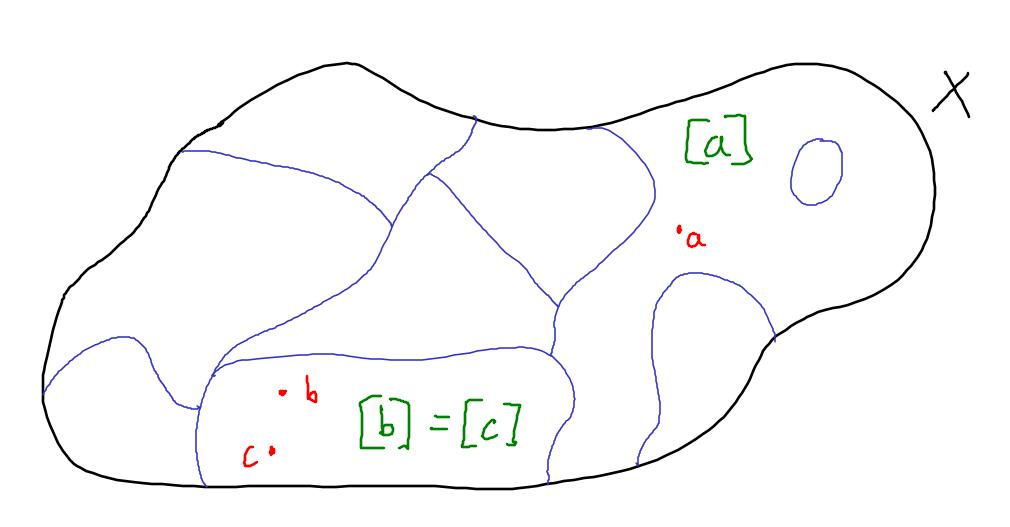
\includegraphics[width=12cm]{./_img/equivalence.jpeg}
        \centering \caption{Die Menge $X$ zerfällt in disjunkte Äquivalenzklassen.}
    \end{figure}
\end{satz}
\begin{proof}
    \begin{labeling}[(P1)]
        \item Per Definition ist jede Äquivalenzklasse eine Teilmenge von $X$. Wegen der Reflexivität gilt für jedes $x\in X$, dass $x\in[x]$, sodass jede Äquivalenzklasse eine nichtleere Menge ist.
        \item Sei $\calP:=X/{\sim}$. Wegen $x\in [x]$ für jedes $x\in X$ ist $X=\bigcup \calP$, und es bleibt zu zeigen, dass die Elemente von $\calP$ paarweise disjunkt sind. Dazu seien $x,y\in X$ beliebig mit $[x]\cap [y]\neq \emptyset$, d.h. es gebe ein Element $a\in [x]\cap [y]$. Dann ist $a\sim x$ und $a\sim y$. Wegen der Symmetrie gilt auch $x\sim a$, und mit der Transitivität folgt aus $x\sim a$ und $a\sim y$, dass $x\sim y$ gilt. Nach \cref{aequiklassegleich} ist dann $[x]=[y]$. \qedhere
    \end{labeling}
\end{proof}


\begin{bem}
    \cref{aequirelvspart} zeigt, dass jede Äquivalenzrelation auf $X$ eine Partition von $X$ induziert. Wir haben also eine Abbildung
        \[ \{ \text{Äquivalenzrelationen auf $X$}\} \to \{ \text{Partitionen von $X$}\} \ ,\ {\sim} \mapsto X/{\sim} \]
    konstruiert. Es lässt sich zeigen, dass diese Abbildung bijektiv ist (versuch es mal!). Die Äquivalenzrelationen auf $X$ stehen also in einer Eins-zu-Eins-Beziehung zu den Partitionen von $X$, beide Konzepte sind „im Wesentlichen gleichwertig“.
    
    Dennoch hat keines der beiden Konzepte Vorrang vor dem Anderen. In den Beispielen mit den Fußballmannschaften und Wohngemeinschaften spielt sicherlich die Partition die „primäre“ Rolle, die aus ihr abgeleiteten Äquivalenzrelationen „wohnt in derselben Wohnung wie“, „spielt im selben Verein wie“ sind hier eher sekundär. In den Beispielen aus \cref{bsp:aequirel} hat dagegen eher die Äquivalenzrelation Vorrang.
\end{bem}





\clearpage
\section{Aufgabenvorschläge}


\begin{aufg}[Eigenschaften von Relationen (L)] \label{aufg:relationen}
    Untersucht die folgenden Relationen darauf, ob sie reflexiv, transitiv, symmetrisch oder antisymmetrisch sind. Welche Relationen sind Ordnungsrelationen, welche Äquivalenzrelationen? Sofern eine Ordnungsrelation vorliegt, versucht, sie mit einem Diagramm zu veranschaulichen.
    \begin{enumerate}
        \item Es bezeichne $S$ die Menge aller Städte auf der Erde. Betrachtet darauf die Relation
        \begin{align*}
            A \sim B \quad& :\Leftrightarrow\quad \text{$A$ und $B$ sind höchstens 100km voneinander entfernt} && A,B\in S
        \end{align*}
        \item Auf der Menge $\R$ die Ungleichheitsrelation $\neq$.
        \item Auf der Menge $\R$ die „strikt kleiner“-Relation $<$.
        \item Auf der Menge $\N$ die Teilbarkeitsrelation:
        \begin{align*}
            m\mid n \qquad:\Leftrightarrow\qquad \exists k\in \N:\ k\cdot m=n && m,n\in \N
        \end{align*}
        \item Sei $X$ eine beliebige Menge. Betrachtet für Folgen $(a_n)_{n\in \N},(b_n)_{n\in \N} \in X^\N$ die Relation:
        \begin{align*}
            (a_n)_{n\in \N} \sim (b_n)_{n\in \N} \qquad & :\Leftrightarrow\qquad \exists N\in \N\ \forall n\in \N_{\ge N}:\ a_n=b_n
        \end{align*}
            Ich sage auch: Die Folgen $(a_n)_{n\in \N},(b_n)_{n\in \N}$ „stimmen überein für hinreichend große $n$“.\footnote{vgl. \cref{def:eventually}}
    \end{enumerate}
\end{aufg}


\begin{aufg}[Schranken (L)] \label{aufg:schranken}
    In dieser Aufgabe geht es um Teilmengen geordneter Mengen. Wir betrachten die geordneten Mengen $(\Q,\le)$ und $(\calP(\N),\subseteq)$ und deren folgende Teilmengen:
    \begin{align*}
        & \text{a)} & \{x\in \Q \mid x\ge 4\} & \subseteq \Q \\
        & \text{b)} & \left\{\tfrac{1}{n}\mid n\in \N_{\ge 1}\right\} & \subseteq \Q \\
        & \text{c)} & \calP(\N)\setminus \{\emptyset\} & \subseteq \calP(\N) \\
        & \text{d)} & \{X\in\calP(\N)\mid X\ \text{enthält nur endlich viele Elemente}\} & \subseteq \calP(\N) \\
        & \text{e)} & \{x\in \Q \mid x^2<2\} & \subseteq \Q
    \end{align*}
    Untersucht jede Teilmenge darauf, ob sie innerhalb der Obermenge nach oben oder unten beschränkt ist, kleinste oder größte, minimale oder maximale Elemente enthält und ob sie innerhalb der Obermenge ein Infimum oder ein Supremum besitzt.
\end{aufg}


\begin{aufg}[Zerlegung der Ebene in Äquivalenzklassen]
    Betrachtet folgende Abbildungen $\R^2\to \R$:
    \begin{align*}
        f_1(x,y) & = y     & f_2(x,y) & = x+y                    & f_3(x,y) & = x^2+y^2 \\
        f_4(x,y) & = xy    & f_5(x,y) & = \lfloor x + y\rfloor   & f_6(x,y) & = \lfloor x^2+y^2\rfloor
    \end{align*}
    \begin{enumerate}
        \item Für jedes $i\in\{1,\dots , 6\}$ zeichnet die Faser $f_i^{-1}(3)$ in die Ebene $\R^2$ ein.
        \item Nach \cref{merkmal} ist für jedes $i\in\{1,\dots , 6\}$ durch
        \begin{align*}
            p\sim_i q \quad &:\Leftrightarrow\quad f_i(p)=f_i(q) && p,q\in \R^2
        \end{align*}
        eine Äquivalenzrelation auf dem $\R^2$ gegeben. Visualisiert die Äquivalenzklassen jeweils mit einer Zeichnung.
    \end{enumerate}
\end{aufg}

